\documentclass[a4paper, 11pt]{article}
%\documentclass{letter}
\usepackage{cmsrb}
\usepackage[OT1,OT2]{fontenc}
\usepackage[utf8]{inputenc}
\usepackage[serbian]{babel}
\usepackage[colorlinks]{hyperref}
\usepackage[left=2.5cm,top=0.5cm,right=1cm, bottom=1.25cm]{geometry} % Document margins
\usepackage{graphicx}
\usepackage{tabularx}
\usepackage{multirow}
\usepackage{ragged2e}
\usepackage{hhline}
\usepackage{array}
\usepackage{amsmath}
\usepackage{xcolor}
\usepackage{tocloft}
\hypersetup{
    urlcolor=blue
}

\renewcommand{\figurename}{Slika}
\renewcommand{\tablename}{Tabela}
\renewcommand{\contentsname}{Sadr\v{z}aj}

\newcommand{\lat}[1]{{\fontencoding{OT1}\selectfont #1}}
\newcommand{\True}{{\fontencoding{OT1}\fontfamily{cmtt}\selectfont\ensuremath{\top}}}
\newcommand{\False}{{\fontencoding{OT1}\fontfamily{cmtt}\selectfont\ensuremath{\bot}}}

\setcounter{tocdepth}{3}

% Define colors
\definecolor{sectioncolor}{RGB}{25, 25, 112}    % Dark blue
\definecolor{subsectioncolor}{RGB}{139, 0, 0}   % Dark red
\definecolor{subsubsectioncolor}{RGB}{0, 100, 0} % Dark green

% Change section color in TOC
\renewcommand{\cftsecfont}{\color{blue}}
\renewcommand{\cftsecpagefont}{\color{blue}}

% Change subsection color in TOC
\renewcommand{\cftsubsecfont}{\color{blue}}
\renewcommand{\cftsubsecpagefont}{\color{blue}}

% Change subsubsection color in TOC
\renewcommand{\cftsubsubsecfont}{\color{blue}}
\renewcommand{\cftsubsubsecpagefont}{\color{blue}}



\begin{document}

\begin{titlepage}
\tableofcontents
\end{titlepage}

\section*{Ulazni parametri potpornog zida}
\addcontentsline{toc}{section}{Ulazni parametri potpornog zida}

\vspace{3cm}

\begin{figure}[h]
    \centering
    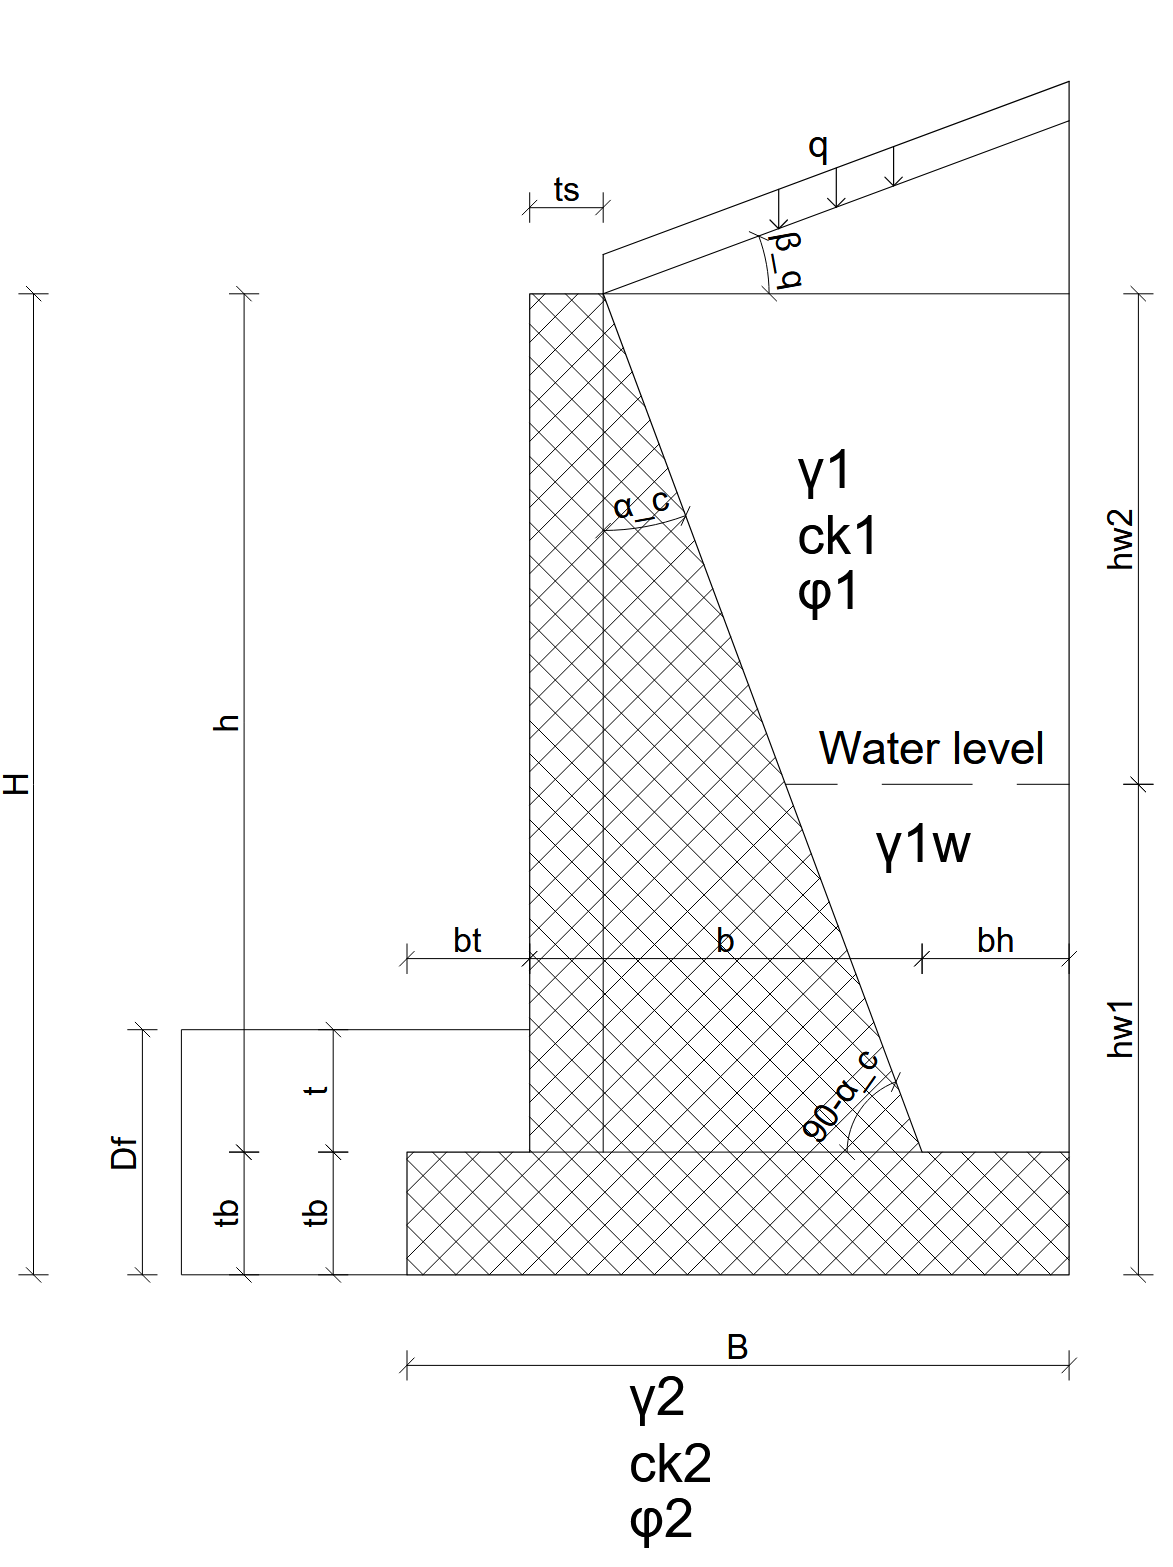
\includegraphics[width=0.8\textwidth, height=15cm]{../Graphics/RetainingWall1_geometry.png}
    \caption{Geometrijiske i mehani\v{c}ke karakteristike potpornog zida}
    \label{geometrija_zida}
\end{figure}

\newpage

\begin{center}
Tabelarni prikaz ulaznih parametara potpornog zida:
\end{center}

\begin{table}[h]
\centering
\begin{minipage}{0.40\textwidth}
\centering
\begin{tabular}{|c|c|c|}
\hline
Parametar & Vrednost & Jedinica mere \\
\hline
$B$ & $B_final$ & $m$ \\
\hline
$h_{w1}$ & $hw1$ & $m$ \\
\hline
$h_{w2}$ & $hw2$ & $m$ \\
\hline
$t_{s}$ & $t_s$ & $m$ \\
\hline
$b_{t}$ & $b_t$ & $m$ \\
\hline
$t_{b}$ & $t_b$ & $m$ \\
\hline
$H$ & $h_u$ & $m$ \\
\hline
$D_{f}$ & $Df$ & $m$ \\
\hline
$b_{h}$ & $b_h$ & $m$ \\
\hline
$b$ & $b_o$ & $m$ \\
\hline
$\beta_{q}$ & $betta_q$ & $\circ$\\
\hline
$\alpha_{c}$ & $alpha_c$ & $\circ$\\
\hline
\end{tabular}
\caption{Geometrijiski parametri potpornog zida}
\label{tab:geometrijiski_parametri}
\end{minipage}
\hfill
\begin{minipage}{0.40\textwidth}
\centering
\begin{tabular}{|c|c|c|}
\hline
Parametar & Vrednost & Jedinica mere \\
\hline
$\gamma_{k,1}$ & $gamma_k_1$ & $kN/m^3$ \\
\hline
$\gamma_{k,2}$ & $gamma_k_2$ & $kN/m^3$ \\
\hline
$\gamma_{k,1,w}$ & $gamma_k1w$ & $kN/m^3$ \\
\hline
$\gamma^{'}$ & $gamma_prime$ & $kN/m^3$ \\
\hline
$\phi_{1}$ & $phi_k_1$ & $\circ$ \\
\hline
$\phi_{2}$ & $phi_k_2$ & $\circ$ \\
\hline
$\sigma_{Rd}$ & $sigma_rd$ & $kPa$ \\
\hline
$\gamma_{c}$ & $gamma_concrete $ & $kN/m^3$ \\
\hline
\end{tabular}
\caption{Mehani\v{c}ki parametri tla u sklopu potpornog zida}
\label{tab:mehanicki_parametri}
\end{minipage}
\end{table}

%\begin{center}
%Tabelarni prikaz optere\'cenja i koeficijenata sigurnosti:
%\end{center}


\begin{table}[h]
\centering
\begin{tabular}{|c|c|c|}
\hline
Parametar & Vrednost & Jedinica mere \\
\hline
$q$ & $ q_u $ & $kN/m^2$ \\
\hline
$\gamma_{g}$ & $ gammag $ & - \\
\hline
$\gamma_{q}$ & $ gammaq $ & - \\
\hline
$\gamma_{g, fav}$ & $ gamma_gfav $ & - \\
\hline
$\gamma_{g, stab}$ & $ gamma_gstb $ & - \\
\hline
$\gamma_{g, dstb}$ & $ gamma_gdstb $ & - \\
\hline
$\gamma_{q, stb}$ & $ gamma_qstb $ & - \\
\hline
$\gamma_{q, dstb}$ & $ gamma_qdstb $ & - \\
\hline
$\gamma_{r,h}$ & $ gamma_rh $ & - \\
\hline
\end{tabular}
\caption{Optere\'cenje $q$ i koeficijenti sigurnosti}
\label{tab:koeficijenti_sigurnosti}
\end{table}

\newpage

\section*{Stati\v{c}ki prora\v{c}un potpornog zida}
\addcontentsline{toc}{section}{Stati\v{c}ki prora\v{c}un potpornog zida}

\subsection*{Pretpostavka o Rankinovoj teoriji ravnih preseka:}
\addcontentsline{toc}{subsection}{Pretpostavka o Rankinovoj teoriji ravnih preseka:}

\noindent Uslov \v{s}iroke pete:

\begin{align*}
b_{h} &\geq (H - t_{b}) \cdot \tan\left(45 - \frac{\phi'_{1,d}}{2}\right)\\
\phi'_{1,d} &= \arctan\left(\frac{\tan(\phi_{1})}{\gamma'_{\phi}}\right) = phi_k_1^\circ \quad \text{gde je } \gamma'_{\phi} = 1\\
b_{h} &\geq (h_u - t_b) \cdot \tan\left(45 - \frac{phi_k_1}{2}\right) = bh_calculated \text{ } [m]
\end{align*}
Usvojena \v{s}irina pete:
\begin{align*}
b_{h} = b_h \text{ } [m]
\end{align*}
Ukupna \v{s}irina temeljne spojnice:
\begin{align*}
B = b_{t} + t_{s} + b_{h} = b_t + t_s + b_h = B_final \text{ } [m]
\end{align*}

\subsection*{Prora\v{c}un uticaja koji deluju na potporni zid:}
\addcontentsline{toc}{subsection}{Prora\v{c}un uticaja koji deluju na potporni zid:}

\begin{figure}[h]
    \centering
    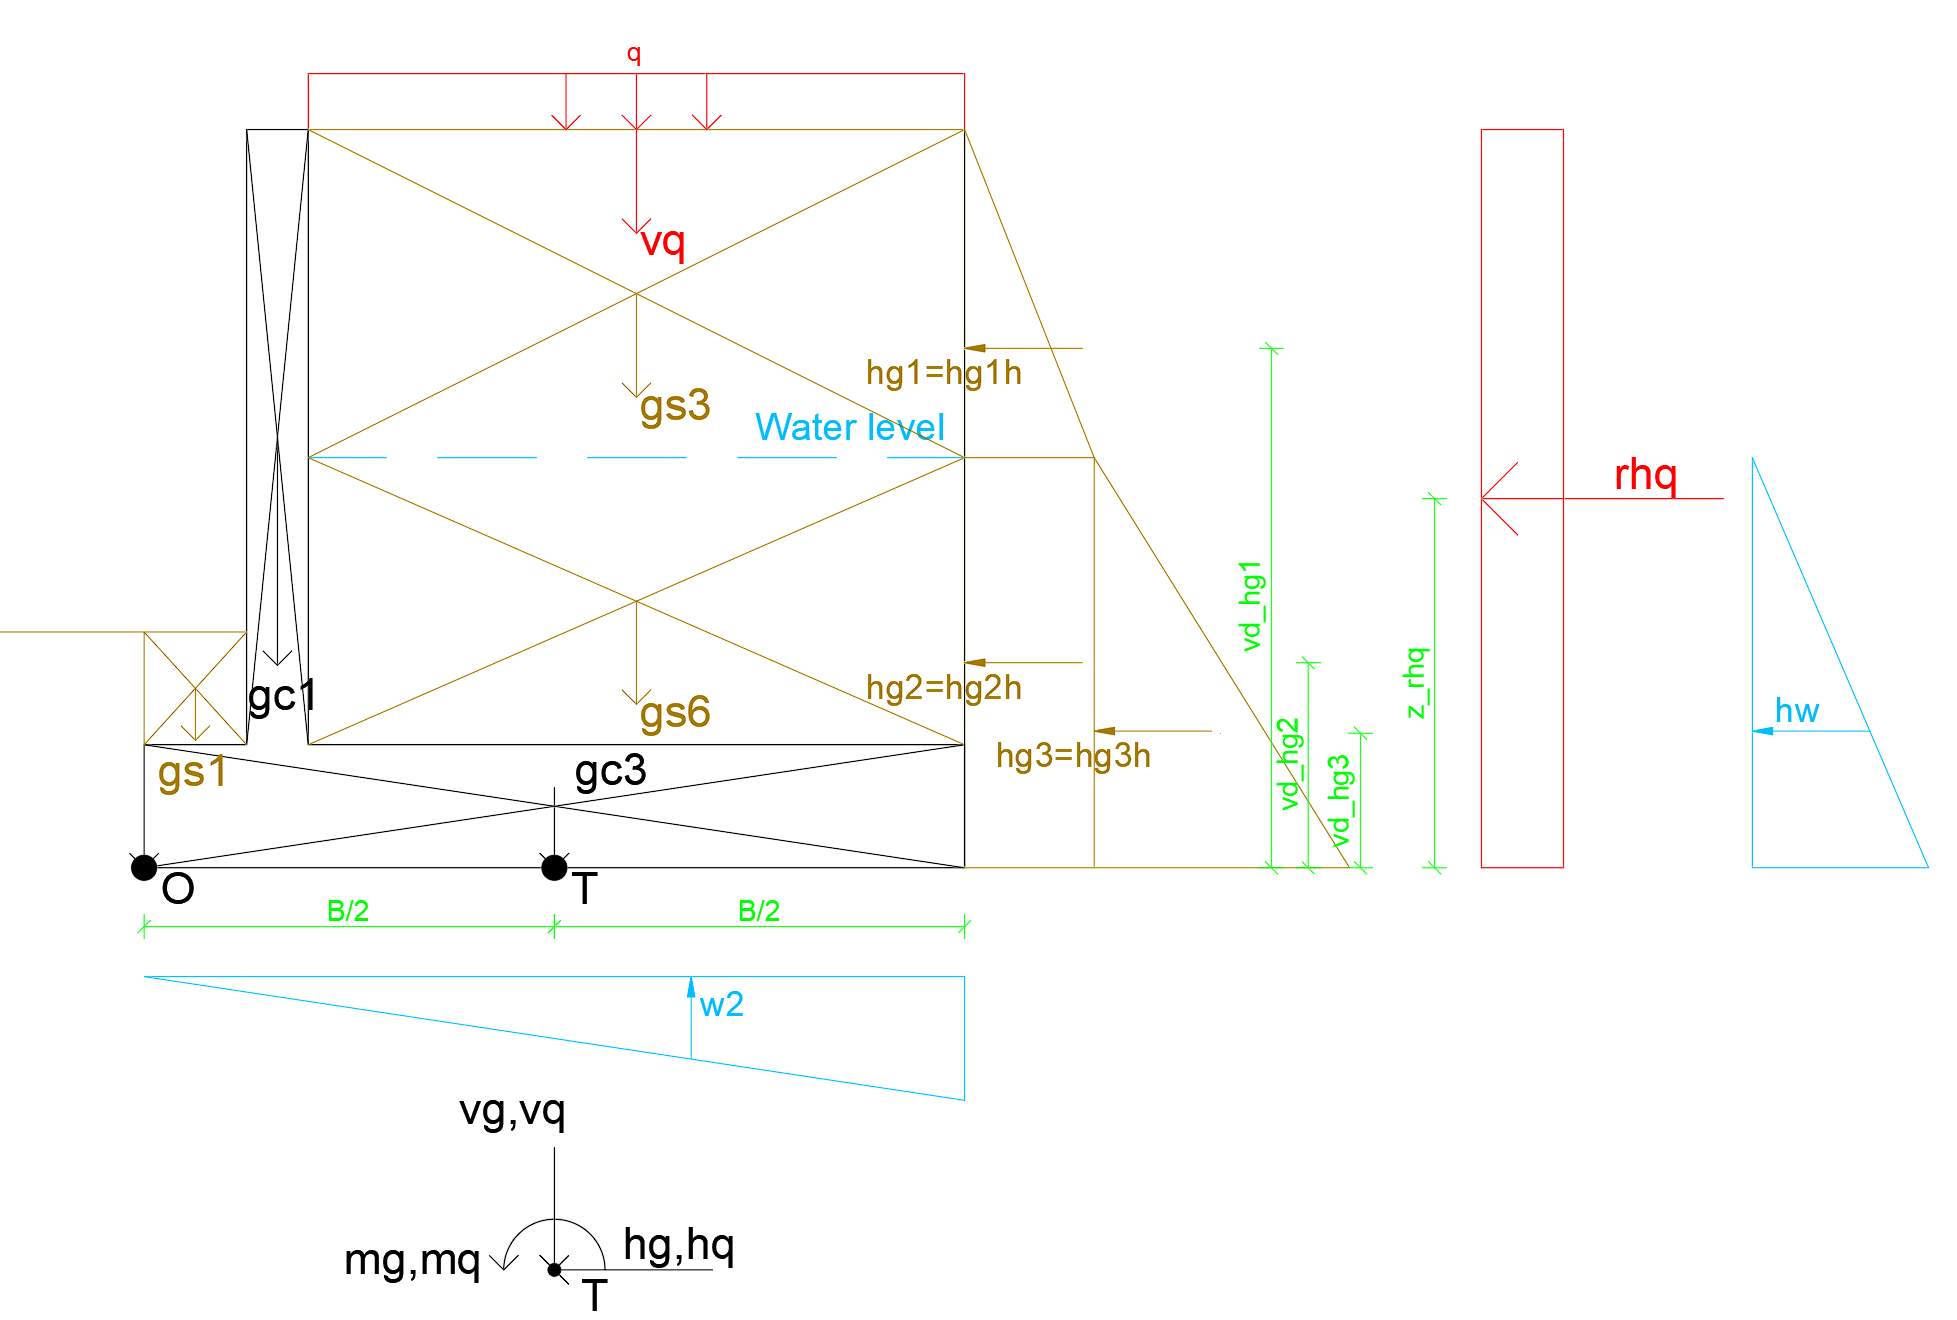
\includegraphics[width=\textwidth, height=15cm]{../Graphics/RetainingWall1_gravity.png}
    \caption{Stati\v{c}ki uticaji na potporni zid od tla, vode i korisnog optere\'cenja}
    \label{uticaji_zida}
\end{figure}


\newpage

\subsection*{Vertikalne komponente optere\'cenja:}
\addcontentsline{toc}{subsection}{Vertikalne komponente optere\'cenja:}


Te\v{z}ina tla $G_{s1}$:

\begin{align*}
G_{s1} = b_{t} \cdot (D_{f} - t_{b}) \cdot \gamma_{k2} = b_t \cdot (Df - t_b) \cdot gamma_k_2 = gs1 \text{ } [kN/m]
\end{align*}

Te\v{z}ina tla $G_{s2}$:

\begin{align*}
G_{s2} = \tan (\alpha_{c}) \cdot \frac{h_{w2}^2}{2} \cdot \gamma_{k,1} = \tan (alpha_c) \cdot \frac{hw2^2}{2} \cdot gamma_k_1 = gs2 \text{ } [kN/m]
\end{align*}

Te\v{z}ina tla $G_{s3}$ (za $h_{w1} \neq 0$):

\begin{align*}
G_{s3} &= (B - b_{t} - t_{s} - \tan{(\alpha_{c})} \cdot h_{w2}) \cdot h_{w2} \cdot \gamma_{k,1} \\
       &= (B_final - b_t - t_s - \tan{alpha_c} \cdot hw2) \cdot hw2 \cdot gamma_k_1 = gs3 \text{ } [kN/m]
\end{align*}

%Te\v{z}ina tla $G_{s3}$ (za $h_{w1} = 0$):
%\begin{align*}
%G_{s3} &= (B - b_{t} - t_{s} - \tan{(\alpha_{c})} \cdot (h_{w2} - t_{b})) \cdot (h_{w2} - t_{b}) * \gamma_{k,1} \\
%	   &= gs_three_eq_zero \text{ } [kN/m]
%\end{align*}

Te\v{z}ina tla $G_{s4}$:

\begin{align*}
G_{s4} &= \tan{(\alpha_{c})} \cdot \frac{(b_{h} + b - t_{s})^2}{2} \cdot \gamma_{k,1} \\
	   &= \tan{(alpha_c)} \cdot \frac{(b_h + b_o - t_s)^2}{2} \cdot gamma_k_1 = gs4 \text{ } [kN/m]
\end{align*}

Te\v{z}ina tla $G_{s5}$:

\begin{align*}
G_{s5} &= \tan{(\alpha_{c})} \cdot \frac{(h_{w1} - t_{b})^2}{2} \cdot \gamma_{k,1,w} \\
       &= \tan{(alpha_c)} \cdot \frac{(hw1 - t_b)^2}{2} \cdot gamma_k1w = gs5 \text{ } [kN/m]
\end{align*}

Te\v{z}ina tla $G_{s6}$ (za $h_{w1} \neq 0$):

\begin{align*}
G_{s6} &= b_{h} \cdot (H - t_{b} - h_{w2}) \cdot \gamma_{k,1,w} \\
       &= b_h \cdot (h_u - t_b - hw2) \cdot gamma_k1w = gs6 \text{ } [kN/m]
\end{align*}

%Te\v{z}ina tla $G_{s6}$ (za $h_{w1} = 0$):

%\begin{align*}
%G_{s6} &= b_{h} \cdot (H - t_{b} - (h_{w2}-t_{b}) \cdot \gamma_{k,1,w} \\
%       &= b_h \cdot (h_u - t_b - (hw2-t_b)) \cdot gamma_k1w = gs_six_eq_zero \text{ } [kN/m]
%\end{align*}

Te\v{z}ina betonskog dela potpornog zida $G_{c1}$:

\begin{align*}
G_{c1} = h \cdot t_{s} \cdot \gamma_{c} = h_prvo \cdot t_s \cdot gamma_concrete = gc1 \text{ } [kN/m]
\end{align*}

Te\v{z}ina betonskog dela potpornog zida $G_{c2}$:

\begin{align*}
G_{c2} &= (B - b_{h} - t_{s} - b_{t}) \cdot (H-t_{b}) \cdot \gamma_{c} \\
	   &= (B_final - b_h - t_s - b_t) \cdot (h_u - t_b) \cdot gamma_concrete = gc2 \text{ } [kN/m]
\end{align*}

Te\v{z}ina betonskog dela potpornog zida $G_{c3}$:

\begin{align*}
G_{c3} = B \cdot t_{b} \cdot \gamma_c = B_final \cdot t_b \cdot gamma_concrete = gc3 \text{ } [kN/m]
\end{align*}

Uzgon $W_{2}$:

\begin{align*}
W_{2} = \frac{(h_{w1} \cdot 9.807) \cdot B}{2} = \frac{(hw1 \cdot 9.807) \cdot B_final}{2} = w_2 \text{ } [kN/m]
\end{align*}
 
 
Korisno optere\'cenje $V_{q}$:

\begin{align*}
\beta_{q} &= betta_q ^\circ \\
V_{q} &= q \cdot  ( B - t_{s} - b_{t}) \cdot \cos(\beta_{q})  \\
      &= q_u \cdot (B_final - t_s - b_t) \cdot \cos(betta_q) = vqq \text{ } [kN/m]
\end{align*}



\subsection*{Koeficijent aktivnog pritiska tla:}
\addcontentsline{toc}{subsection}{Koeficijent aktivnog pritiska tla:}

Koeficijent aktivnog pritiska tla $K_{a}$:

\begin{align*}
\beta_{q} &= betta_q ^\circ \\
\phi'_{d1} &= phi_prime1d ^\circ  \\
k_a &= \frac{\cos(\beta_q) - \sqrt{\sin^2(\phi'_{d1}) - \sin^2(\beta_q)}}{\cos(\beta_q) + \sqrt{\sin^2(\phi'_{d1}) - \sin^2(\beta_q)}} \\
	&= koeficijent_ka
\end{align*}

\subsection*{Komponente optere\'cenja pod uglom $\beta_{q} = betta_q ^ \circ$}
\addcontentsline{toc}{subsection}{Komponente optere\'cenja pod uglom $\beta_{q} = betta_q ^ \circ$}

Komponenta optere\'cenja $H_{g1}$ pod uglom $\beta_{q} = betta_q ^ \circ$:

\begin{align*}
H_{g1} &= \frac{\gamma_{k1} \cdot \left(h_{w2} \right)^2 \cdot K_{a} \cdot \cos(\beta_q)}{2}\\
	   &=  \frac{gamma_k_1 \cdot \left(hw2 \right)^2 \cdot koeficijent_ka \cdot \cos(betta_q)}{2} \\
	   &= h_g1 \text{ } [kN/m] \\
\end{align*}

Komponenta optere\'cenja $H_{g2}$ pod uglom $\beta_{q} = betta_q ^ \circ$:
\begin{align*}
H_{g2} &= \gamma_{k1} \cdot h_{w2}^2 \cdot K_{a} \cdot \cos(\beta_{q}) \cdot h_{w1} \\
	   &= gamma_k_1 \cdot hw2^2 \cdot koeficijent_ka \cdot \cos (betta_q) \cdot hw1 \\
	   &= h_g2 \text{ } [kN/m]
\end{align*}

Komponenta optere\'cenja $H_{g3}$ pod uglom $\beta_{q} = betta_q ^ \circ$:

\begin{align*}
\gamma_{k1w} &= gamma_k1w \text{ } kN/m^3 \\
\gamma' &= \gamma_{k1w} - 9.807 \text{ za } h_{w1} \neq 0 \text{; u suprotnom } \gamma' = \gamma_{k1} \\
H_{g3}  &= \frac{\gamma' \cdot h_{w1} ^2 \cdot K_{a} \cdot \cos( \beta_{q})}{2} \\
		&= \frac{gamma_prime \cdot hw1 ^2 \cdot koeficijent_ka \cdot \cos(betta_q)}{2} \\
		&= h_g3 \text{ } [kN/m]
\end{align*}

Komponenta optere\'cenja $H_{q}$ pod uglom $\beta_{q} = betta_q ^ \circ$:

\begin{align*}
H_{q} &=   \left(q \cdot K_{a} \cdot ((B - b_{t} - t_{s}) \cdot \tan (\beta_q) + h_{w1} + h_{w2}) \right) \cdot \cos(\beta_{q})  \\
	  &= \left( q_u \cdot koeficijent_ka \cdot ((B_final - b_t - t_s) \cdot \tan (betta_q) + hw1 + hw2) \right) \cdot \cos(betta_q)  \\
	  &= hqq \text{ } [kN/m]
\end{align*}

Komponenta optere\'cenja $H_{w}$ (pod uglom $\beta=0^\circ$):

\begin{align*}
H_{w} &=  \frac{h_{w1}^2 \cdot 9.807}{2} \\
      &= \frac{hw1^2 \cdot 9.807}{2} \\
      &= h_w \text{ } [kN/m]
\end{align*}

\subsection*{Rastojanja horizontalnih i vertikalnih komponenti optere\'cenja od te\v{z}i\v{s}ta $T$($v$ - vertikalno rastojanje, $h$ - horizontalno rastojanje)}
\addcontentsline{toc}{subsection}{Rastojanja horizontalnih i vertikalnih komponenti optere\'cenja od te\v{z}i\v{s}ta $T$($v$ - vertikalno rastojanje, $h$ - horizontalno rastojanje)}

\begin{align*}
h_{d,Hg1} &= h_{d,Hg2} = h_{d,Hg3} = h_{d,Hq}  = \frac{B}{2} = \frac{B_final}{2} = hd_hg1 \text{ } [m]\\
v_{d,Hg1} &= h_{w1} + \frac{1}{3} \cdot \left[(B - b_{t} - t_{s}) \cdot \tan(\beta_{q}) + h_{w2}\right] \\
         &= hw1 + \frac{1}{3} \cdot \left[(B_final - b_t - t_s) \cdot \tan(betta_q) + hw2 \right] \\
         &= vd_hg1 \text{ } [m] \\
v_{d,Hg2} &= \frac{h_{w1}}{2} = \frac{hw1}{2} =  vd_hg2 \text{ } [m] \\
v_{d,Hg3} &=  \frac{h_{w1}}{3} = \frac{hw1}{3} =  vd_hg3 \text{ } [m] \\
v_{d,Hw} &= \frac{h_{w1}}{3} = \frac{hw1}{3} =  vd_hw \text{ } [m] \\
v_{d,Hq} &= \frac{(B - b_{t} - t_{s}) \cdot \tan(\beta_{q}) + h_{w2} + h_{w1}}{2} \\
		&= \frac{(B_final - b_t - t_s) \cdot \tan(betta_q) + hw2 + hw1}{2} \\
		&= vd_hq \text{ } [m]
\end{align*}

\subsection*{Suma vertikalnih komponenti optere\'cenja:}
\addcontentsline{toc}{subsection}{Suma vertikalnih komponenti optere\'cenja}

\begin{align*}
V_{g,u} &= \sum_{i=1}^{3} H_{gi} \cdot \sin(\beta_{q}) + \sum_{i=1}^3 {G_{ci}} + \sum_{i=1}^{6} {G_{si}} -W_{2} \\
		&= \left( h_g1 + h_g2 + h_g3 \right) \cdot sin(betta_q)+  \\
		&= gc1+gc2+gc3 + \\
		&= gs1+gs2+gs3+gs4+gs5+gs6 - w2 \\
		&= v_gu \text{ } [kN/m] \\
V_{q,u} &= V_{q} + H_{q} \cdot \sin(\beta_{q}) \\
		&= vqq + hqq \cdot \sin (betta_q) \\
		&= v_qu \text{ } [kN/m]
\end{align*}

\subsection*{Suma horizontalnih komponenti optere\'cenja:}
\addcontentsline{toc}{subsection}{Suma horizontalnih komponenti optere\'cenja}

\begin{align*}
H_{g,u} &= \sum_{i=1}^{3} H_{gi} \cdot \cos(\beta_{q}) + H_{w} \\
		&=  \left( h_g1 + h_g2 + h_g3 \right) \cdot \cos (betta_q) + h_w \\
		&= h_gu \text{ } [kN/m] \\
H_{q,u} &= H_{q} \cdot \cos (\beta_{q}) \\
		&= hqq \cdot \cos (betta_q) \\
		&= h_qu \text{ } [kN/m]
\end{align*}

\subsection*{Svo\dj enje optere\'cenja na te\v{z}i\v{s}te temeljne spojnice T:}
\addcontentsline{toc}{subsection}{Svo\dj enje optere\'cenja na te\v{z}i\v{s}te temeljne spojnice T}
Vertikalne komponente:
\begin{align*}
\left[V_{g,u}, V_{q,u} \right] = \left[v_gu, v_qu \right] \text{ } [kN/m]
\end{align*}
Horizontalne komponente:
\begin{align*}
\left[ H_{g,u}, H_{q,u} \right] = \left[ h_gu, h_qu \right] \text{ } [kN/m]
\end{align*}

Momenat od stalnog optere\'cenja u te\v{z}i\v{s}tu T (pozitivan znak je u smeru kazaljke na satu):

\begin{align*}
M_{g} &= G_{c1} \cdot \left( \frac{B}{2} - b_{t} - \frac{t_{s}}{2} \right) +  \\
   &\quad G_{c2} \cdot \left( \frac{B}{2} - b_{t} - t_{s} - \frac{b - t_{s}}{3} \right) + \\
   &\quad G_{c3} \cdot \left( \frac{B}{2} - \frac{B}{2} \right) + \\
   &\quad G_{s1} \cdot \left( \frac{B}{2} - \frac{b_{t}}{2} \right) + \\
   &\quad G_{s2} \cdot \left( \frac{B}{2} - b_{t} - t_{s} - \frac{2}{3} \cdot \tan (\alpha_{c}) \cdot h_{w2} \right) - \\
   &\quad G_{s3} \cdot \left( \frac{b_{t} + t_{s} + \tan (\alpha_{c}) \cdot h_{w2}}{2}  \right) - \\
   &\quad G_{s4} \cdot \left( \frac{B}{2} - \frac{B - b_{t} - t_{s}}{3} \right) + \\
   &\quad G_{s5} \cdot \left( \frac{B}{2} - \left(b_{t} + t_{s} + \tan(\alpha_{c}) \cdot h_{w2} + \frac{2}{3} \left(b - t_{s} - \tan(\alpha_{c}) \cdot h_{w2} \right)\right) \right) - \\
   &\quad G_{s6} \cdot \left( \frac{B}{2} - \frac{B}{3} \right) + \\
   &\quad H_{g1} \cdot  \left( \cos (\beta_{q}) \cdot v_{d,Hg1} -  \sin (\beta_{q}) \cdot h_{d,Hg1} \right) + \\
   &\quad H_{g2} \cdot \left( \cos (\beta_{q}) \cdot v_{d,Hg2} -  \sin (\beta_{q}) \cdot h_{d,Hg2} \right) +  \\
   &\quad H_{g3} \cdot \left( \cos (\beta_{q}) \cdot v_{d,Hg3} -  \sin (\beta_{q}) \cdot h_{d,Hg3} \right) +  \\
   &\quad H_{w} \cdot \frac{h_{w1}}{3} + \\
   &\quad W_2 \cdot \left( \frac{B}{2} - \frac{B}{3} \right) \\
M_{g} &= gc1 \cdot \left( \frac{B_final}{2} - b_t - \frac{t_s}{2} \right) +  \\
   &\quad gc2 \cdot \left( \frac{B_final}{2} - b_t - t_s - \frac{b - t_s}{3} \right) + \\
   &\quad gc3 \cdot \left( \frac{B_final}{2} - \frac{B_final}{2} \right) + \\
   &\quad gs1 \cdot \left( \frac{B_final}{2} - \frac{b_t}{2} \right) + \\
   &\quad gs2 \cdot \left( \frac{B_final}{2} - b_t - t_s - \frac{2}{3} \cdot \tan (alpha_c) \cdot hw2 \right) - \\
   &\quad gs3 \cdot \left( \frac{b_t + t_s + \tan (alpha_c) \cdot hw2}{2}  \right) - \\
   &\quad gs4 \cdot \left( \frac{B_final}{2} - \frac{B_final - b_t - t_s}{3} \right) + \\
   &\quad gs5 \cdot \left( \frac{B_final}{2} - \left(b_t + t_s + \tan(alpha_c) \cdot hw2 + \frac{2}{3} \left(b - t_s - \tan(alpha_c) \cdot hw2 \right)\right) \right) - \\
   &\quad gs6 \cdot \left( \frac{B_final}{2} - \frac{B_final}{3} \right) + \\
   &\quad h_g1 \cdot  \left( \cos (betta_q) \cdot vd_hg1 -  \sin (betta_q) \cdot hd_hg1 \right) + \\
   &\quad h_g2 \cdot \left( \cos (betta_q) \cdot vd_hg2 -  \sin (betta_q) \cdot hd_hg1 \right) +  \\
   &\quad h_g3 \cdot \left( \cos (betta_q) \cdot vd_hg3 -  \sin (betta_q) \cdot hd_hg1 \right) +  \\
   &\quad h_w \cdot \frac{hw1}{3} + \\
   &\quad w_2 \cdot \left( \frac{B_final}{2} - \frac{B_final}{3} \right) \\
M_{g} &= m_g \text{ } [kNm/m]
\end{align*}

Momenat od korisnog optere\'cenja u te\v{z}i\v{s}tu T (pozitivan znak je u smeru kazaljke na satu):

\begin{align*}
M_{q} &= H_{q} \cdot \cos (\beta_{q}) \cdot v_{d,Hq} - \\
	  &\quad H_{q} \cdot \sin (\beta_{q}) \cdot h_{d,Hq} - \\	
	  &\quad q \cdot (B - b_{t} - t_{s}) \cdot h_{d,Q} \\
M_{q} &= hqq \cdot \cos (betta_q) \cdot vd_hq - \\
	  &\quad hqq \cdot \sin (betta_q) \cdot hd_hg1 - \\	
	  &\quad q_u \cdot (B_final - b_t - t_s) \cdot hd_q \\
M_{q} &= m_q \text{ } [kNm/m]
\end{align*}

\subsection*{Prora\v{c}un maksimalnog i minimalnog bruto napona na ivicama temeljne spojnice \lat{ULS STR}:}
\addcontentsline{toc}{subsection}{Prora\v{c}un maksimalnog i minimalnog bruto napona na ivicama temeljne spojnice \lat{ULS STR}}

\begin{align*}
B &= B_final \text{ } [m] \\
V_{g} &= v_gu \text{ } [kN/m] \\
V_{q} &= v_qu \text{ } [kN/m] \\
m_{g} &= m_g \text{ } [kNm/m] \\
m_{q} &= m_q \text{ } [kNm/m] \\
F &= B \cdot 1 = B_final \cdot 1 = area_of_footing \text{ } [m^2] \\
W &= \frac{B^2 \cdot 1}{6} = \frac{B_final ^ 2 \cdot 1}{6} = section_modulus \text{ } [m^3]  \\
V_{Ed} &= \gamma_{g} \cdot V_{g} + \gamma_{q} \cdot V_{q} \\
	   &= gammag \cdot v_gu + gammaq \cdot v_qu \\
	   &= ved_gross \text{ } [kN/m]\\
M_{Ed} &= \gamma_{g} \cdot M_{g} + \gamma_{q} \cdot M_{q} \\
	   &= gammag \cdot m_g + gammaq \cdot m_q \\
	   &= med_gross \text{ } [kNm/m]
\end{align*}

\subsubsection*{Maksimalni bruto kontaktni napon $\sigma_{max}$:}
\addcontentsline{toc}{subsection}{Maksimalni bruto kontaktni napon $\sigma_{max}$}

\begin{align*}
\sigma_{max} &= \frac{V_{Ed}}{F} + \frac{M_{Ed}}{W} \\
             &= \frac{ved_gross}{area_of_footing} + \frac{med_gross}{section_modulus} \\
             &= sigma_max_gross \text{ } [\frac{kPa}{m}]
\end{align*}

\subsubsection*{Minimalni bruto kontaktni napon $\sigma_{min}$:}
\addcontentsline{toc}{subsection}{Minimalni bruto kontaktni napon $\sigma_{min}$}

\begin{align*}
\sigma_{min} &= \frac{V_{Ed}}{F} - \frac{M_{Ed}}{W} \\
             &= \frac{ved_gross}{area_of_footing} - \frac{med_gross}{section_modulus} \\
             &= sigma_min_gross \text{ } [\frac{kPa}{m}]
\end{align*}

\subsection*{Kontrola maksimalnog i minimalnog bruto napona na ivicama temeljne spojnice \lat{ULS STR}:}
\addcontentsline{toc}{subsection}{Kontrola maksimalnog i minimalnog bruto napona na ivicama temeljne spojnice \lat{ULS STR}}
\subsubsection*{Kontrola maksimalnog bruto kontaktnog napona $\sigma_{max}$:}
\addcontentsline{toc}{subsubsection}{Kontrola maksimalnog bruto kontaktnog napona $\sigma_{max}$}

\begin{align*}
\sigma_{max} &\leq \sigma_{Rd} \quad [\frac{kPa}{m}] \\
sigma_max_gross &\leq sigma_rd  \quad \rightarrow \left( \lat{\texttt{max_gross_stress_check}} \right)
\end{align*}

\subsubsection*{Kontrola minimalnog bruto kontaktnog napona $\sigma_{min}$:}
\addcontentsline{toc}{subsubsection}{Kontrola minimalnog bruto kontaktnog napona $\sigma_{min}$}
\begin{align*}
\sigma_{min} &\geq 0 \quad [\frac{kPa}{m}] \\
sigma_min_gross &\geq 0  \quad \rightarrow \left( \lat{\texttt{min_gross_stress_check}} \right)
\end{align*}

\subsection*{Kontrola stabilnosti potpornog zida na preturanje:}
\addcontentsline{toc}{subsection}{Kontrola stabilnosti potpornog zida na preturanje}
\subsubsection*{Parametri u zavisnosti od dimenzije $b$ (zavisi od kosine zale\dj a potpornog zida):}
\addcontentsline{toc}{subsubsection}{Parametri u zavisnosti od dimenzije $b$ (zavisi od kosine zale\dj a potpornog zida)}

\begin{align*}
b &= bb \text{ } [m] \\
&\rightarrow param = paramm \text{ } [m] \\
&\rightarrow param_{q} = paramq \text{ } [m] 
\end{align*}

\noindent Stabili\v{s}u\'ci moment se ra\v{c}una oko ta\v{c}ke $O$, stabili\v{s}u\'cim momentom se smatra onim \v{c}iji je smer suprotan od smera kazaljke na satu. Destabili\v{s}u\'ci momentom se smatra moment suprotnog smera od stabili\v{s}u\'ceg. \\
Za stabilnost se koristi redukovan ugao $\phi'_d$ i njemu shodno korigovan koeficijent aktivnog pritiska tla $K_{a,stb}$:

\begin{align*}
\tan (\phi'_d) = \frac{\tan(\phi'_1)}{\gamma_{\phi}}; \quad \gamma_{\phi} = 1.25 \quad \rightarrow \phi'_{d1,stb} = phi_prime_stab_1 ^\circ
\end{align*}

Pa je koeficijent aktivnog pritiska tla:

\begin{align*}
K_{a,stb} = kstb_1
\end{align*}

Vrednosti $H_{gi}$ su sra\v{c}unate za vrednost $K_{a,stb} = kstb_1$.

\subsubsection*{Stabili\v{s}u\'ci moment $M_{Ed,stb}$:}
\addcontentsline{toc}{subsubsection}{Stabili\v{s}u\'ci moment $M_{Ed,stb}$}

\begin{align*}
M_{Ed,stb} &= \gamma_{g,stab} \cdot \bigg[ \\
		   &\quad G_{c1} \cdot \left( \frac{t_{s}}{2} + b_{t} \right) + G_{c2} \cdot \left( \frac{b - t_{s}}{3} + b_{t} + t_{s} \right) + G_{c3} \cdot \left( \frac{B}{2} \right) + \\
		   &\quad G_{s1} \cdot \left( \frac{b_{t}}{2} \right) + G_{s2} \cdot \left( \frac{2}{3} \cdot \tan(\alpha_{c}) \cdot h_{w2} + t_{s} + b_{t} \right) + \\
		   &\quad G_{s3} \cdot \left( \frac{B + \tan(\alpha_{c}) \cdot h_{w2} + t_{s} + b_{t}}{2} \right) + G_{s4} \cdot \left( \frac{2}{3} \cdot (B - b_{t} - t_{s}) + t_{s} + b_{t} \right) + \\
		   &\quad G_{s5} \cdot \left( b_{t} + t_{s} + \tan(\alpha_{c}) \cdot h_{w2} + \frac{2}{3} \cdot (h_{w1} - t_{b}) \cdot \tan(\alpha_{c})\right) + G_{s6} \cdot \left( \frac{b_{h}}{2} + b + b_{t} \right) + \\
		   &\quad H_{g1,stab} \cdot \sin(\beta_{q}) \cdot B + H_{g2,stab} \cdot \sin(\beta_{q}) \cdot B + H_{g3,stab} \cdot \sin(\beta_{q}) \cdot B \bigg] + \\
		   &\quad \gamma_{q,stab} \cdot \bigg[ H_{q} \cdot \sin(\beta_{q}) \cdot B + V_{q} \cdot param_{q} \bigg] \\
\end{align*} 
\begin{align*}
M_{Ed,stb} &= gamma_gstb \cdot \bigg[ \\
		   &\quad gc1 \cdot \left( \frac{t_s}{2} + b_t \right) + gc2 \cdot \left( \frac{bb - t_s}{3} + b_t + t_s \right) + gc3 \cdot \left( \frac{B_final}{2} \right) + \\
		   &\quad gs1 \cdot \left( \frac{b_t}{2} \right) + gs2 \cdot \left( \frac{2}{3} \cdot \tan(alpha_c) \cdot hw2 + t_s + b_t \right) + \\
		   &\quad gs3 \cdot \left( \frac{B_final + \tan(alpha_c) \cdot hw2 + t_s + b_t}{2} \right) + gs4 \cdot \left( \frac{2}{3} \cdot (B_final - b_t - t_s) + t_s + b_t \right) + \\
		   &\quad gs5 \cdot \left( b_t + t_s + \tan(alpha_c) \cdot hw2 + \frac{2}{3} \cdot (hw1 - t_b) \cdot \tan(alpha_c)\right) + gs6 \cdot \left( \frac{b_h}{2} + bb + b_t \right) + \\
		   &\quad hg1_stab \cdot \sin(betta_q) \cdot B_final + hg2_stab \cdot \sin(betta_q) \cdot B_final + hg3_stab \cdot \sin(betta_q) \cdot B_final \bigg] + \\
		   &\quad gamma_qstb \cdot \bigg[ hqq \cdot \sin(betta_q) \cdot B_final + vqq \cdot paramq \bigg] = med_stb \text{ } [kNm/m] \\	   
\end{align*}

\subsubsection*{Destabili\v{s}u\'ci moment $M_{Ed,dstb}$:}
\addcontentsline{toc}{subsubsection}{Destabili\v{s}u\'ci moment $M_{Ed,dstb}$}

\begin{align*}
M_{Ed,dstb} &= \gamma_{g,dstb} \cdot \bigg[ \\
		   &\quad H_{g1} \cdot \cos(\beta_{q}) \cdot \left( h_{w1} + \tan(\beta_{q}) \cdot param + \frac{h_{w2}}{3} \right) + \\
		   &\quad H_{g2} \cdot \cos(\beta_{q}) \cdot \frac{h_{w1}}{2} + H_{g3} \cdot \cos(\beta_{q}) \cdot \frac{h_{w1}}{3} + \\
		   &\quad W_{2} \cdot \frac{2}{3} \cdot B + H_{w} \cdot \frac{h_{w1}}{3} \bigg] + \\
		   &\quad \gamma_{q,dstb} \cdot H_{q} \cdot \cos(\beta_{q}) \cdot \frac{H + \tan(\beta_{q}) \cdot (b_{h} + b - t_{s})}{2}
\end{align*}

\begin{align*}
M_{Ed,dstb} &= gamma_gdstb \cdot \bigg[ \\
		   &\quad h_g1 \cdot \cos(betta_q) \cdot \left( hw1 + \tan(betta_q) \cdot paramm + \frac{hw2}{3} \right) + \\
		   &\quad h_g2 \cdot \cos(betta_q) \cdot \frac{hw1}{2} + h_g3 \cdot \cos(betta_q) \cdot \frac{hw1}{3} + \\
		   &\quad w_2 \cdot \frac{2}{3} \cdot B_final + h_w \cdot \frac{hw1}{3} \bigg] + \\
		   &\quad gamma_qdstb \cdot hqq \cdot \cos(betta_q) \cdot \frac{h_u + \tan(betta_q) \cdot (b_h + b - t_s)}{2} = med_dstb \text{ } [kNm/m] 
\end{align*}

Kontrola stabilnosti potpornog zida na preturanje:

\begin{align*}
M_{Ed,dstb} &\leq M_{Ed,stb} \text{ } [kNm/m] \\
med_dstb &\leq med_stb \quad \left( overturning_stability_check \right)
\end{align*}

\subsection*{Kontrola potpornog zida na klizanje temeljne spojnice:}
\addcontentsline{toc}{subsection}{Kontrola potpornog zida na klzanje temeljne spojnice}

\begin{align*}
V_{g} &= \gamma_{g,fav} \cdot \left( \sum_{i=1} ^ 3 G_{ci} + \sum_{i=1} ^ 6  G_{si} + W_{2} \right) - W_{2} \cdot \gamma_{g} \\
V_{q} &= \gamma_{q} \cdot V_{q} \\
V_{d} &= V_{g} + V_{q} \\
H_{Rd} &= \frac{V_{d} \cdot \tan(\phi'_2)}{\gamma_{r,h}} \\
H_{d} &= \gamma_g \cdot \left( H_{g1} \cdot \cos(\beta_{q}) + H_{g2} \cdot \cos(\beta_{q}) + H_{g3} \cdot \cos(\beta_{q}) + H_{w} \right) + \\
    &\quad \gamma_{q} \cdot H_{q} \cdot \cos(\beta_{q})
\end{align*}

\begin{align*}
V_g &= gamma_gfav \cdot \left( gc1+gc2+gc3+gs1+gs2+gs3+gs4+gs5+gs6 + w_2 \right) - w_2 \cdot gammag = vg_slide \text{ } [kN/m] \\
V_q &= gammaq \cdot v_qu = vq_slide \text{ } [kN/m] \\
V_d &= vg_slide + vq_slide = vd_slide \text{ } [kN/m] \\
H_{Rd} &= \frac{vd_slide \cdot \tan(phi_prime_stab_2)}{gamma_rh} = hrd_slide \text{ } [kN/m] \\
H_d &= gammag \cdot \left( h_g1 \cdot \cos(betta_q) + h_g2 \cdot \cos(betta_q) + h_g3 \cdot \cos(betta_q) \right) + \\
    &\quad gammag \cdot h_w + gammaq \cdot hqq \cdot \cos(betta_q) = hd_slide \text{ } [kN/m]
\end{align*}

Kontrola potpornog zida na klizanje temeljne spojnice:

\begin{align*}
H_{d} \leq H_{Rd} \text{ } [kN/m]  \\
hd_slide \leq hrd_slide \quad \left( sliding_check \right)
\end{align*}

\subsection*{Rekapitulacija kontrola potpornog zida:}
\addcontentsline{toc}{subsection}{Rekapitulacija kontrola potpornog zida}
\subsubsection*{Kontrola maksimalnog i minimalnog napona na temeljnoj spojnici:}
\addcontentsline{toc}{subsubsection}{Kontrola maksimalnog i minimalnog napona na temeljnoj spojnici}

\begin{align*}
\sigma_{max} &\leq \sigma_{Rd} \quad [\frac{kPa}{m}] \\
sigma_max_gross &\leq sigma_rd  \quad \rightarrow \left( \lat{\texttt{max_gross_stress_check}} \right)\\
\sigma_{min} &\geq 0 \quad [\frac{kPa}{m}] \\
sigma_min_gross &\geq 0  \quad \rightarrow \left( \lat{\texttt{min_gross_stress_check}} \right)
\end{align*}

\subsubsection*{Kontrola stabilnosti potpornog zida na preturanje:}
\addcontentsline{toc}{subsubsection}{Kontrola stabilnosti potpornog zida na preturanje}
\begin{align*}
M_{Ed,dstb} &\leq M_{Ed,stb} \text{ } [kNm/m] \\
med_dstb &\leq med_stb \quad \left( overturning_stability_check \right)
\end{align*}

\subsubsection*{Kontrola potpornog zida na klizanje temeljne spojnice:}
\addcontentsline{toc}{subsubsection}{Kontrola potpornog zida na klizanje temeljne spojnice}
\begin{align*}
H_{d} \leq H_{Rd} \text{ } [kN/m]  \\
hd_slide \leq hrd_slide \quad \left( sliding_check \right)
\end{align*}

\end{document}